% =============================================================
%  CHAPITRE 7 : TUTEUR CONVERSATIONNEL (v2)
% =============================================================
\section{Évolution vers un tuteur conversationnel (v2)}
\label{sec:tuteur-v2}

\subsection{Motivation}

Le système présenté dans les chapitres précédents (v1) fonctionne en mode questions-réponses direct : chaque question est traitée indépendamment, sans mémoire des échanges antérieurs. L'étudiant ne peut pas poser de questions de suivi naturelles sans que le système perde le contexte. De plus, la posture est purement transmissive : le système répond directement, sans guidage socratique ni adaptation du niveau.

La version 2 transforme ce moteur Q\&A en un véritable \textbf{tuteur conversationnel} en ajoutant quatre capacités fondamentales :

\begin{enumerate}
  \item Une \textbf{mémoire de conversation} avec compression automatique pour gérer un historique multi-tours ;
  \item Un \textbf{prompt socratique} qui guide l'étudiant par des relances plutôt que de fournir la réponse ;
  \item Le \textbf{streaming} token par token pour une expérience interactive fluide ;
  \item Une \textbf{évaluation en temps réel} par question pour diagnostiquer la qualité du retrieval et de la génération.
\end{enumerate}

L'architecture modulaire du pipeline a permis d'ajouter ces capacités sans modifier le cœur du système : \texttt{pipeline.answer()} acceptait déjà les paramètres \texttt{history} et \texttt{system\_prompt} de manière optionnelle. La v2 les exploite pleinement.

\subsection{Architecture de la mémoire conversationnelle}
\label{sec:memoire-archi}

\begin{figure}[H]
\centering
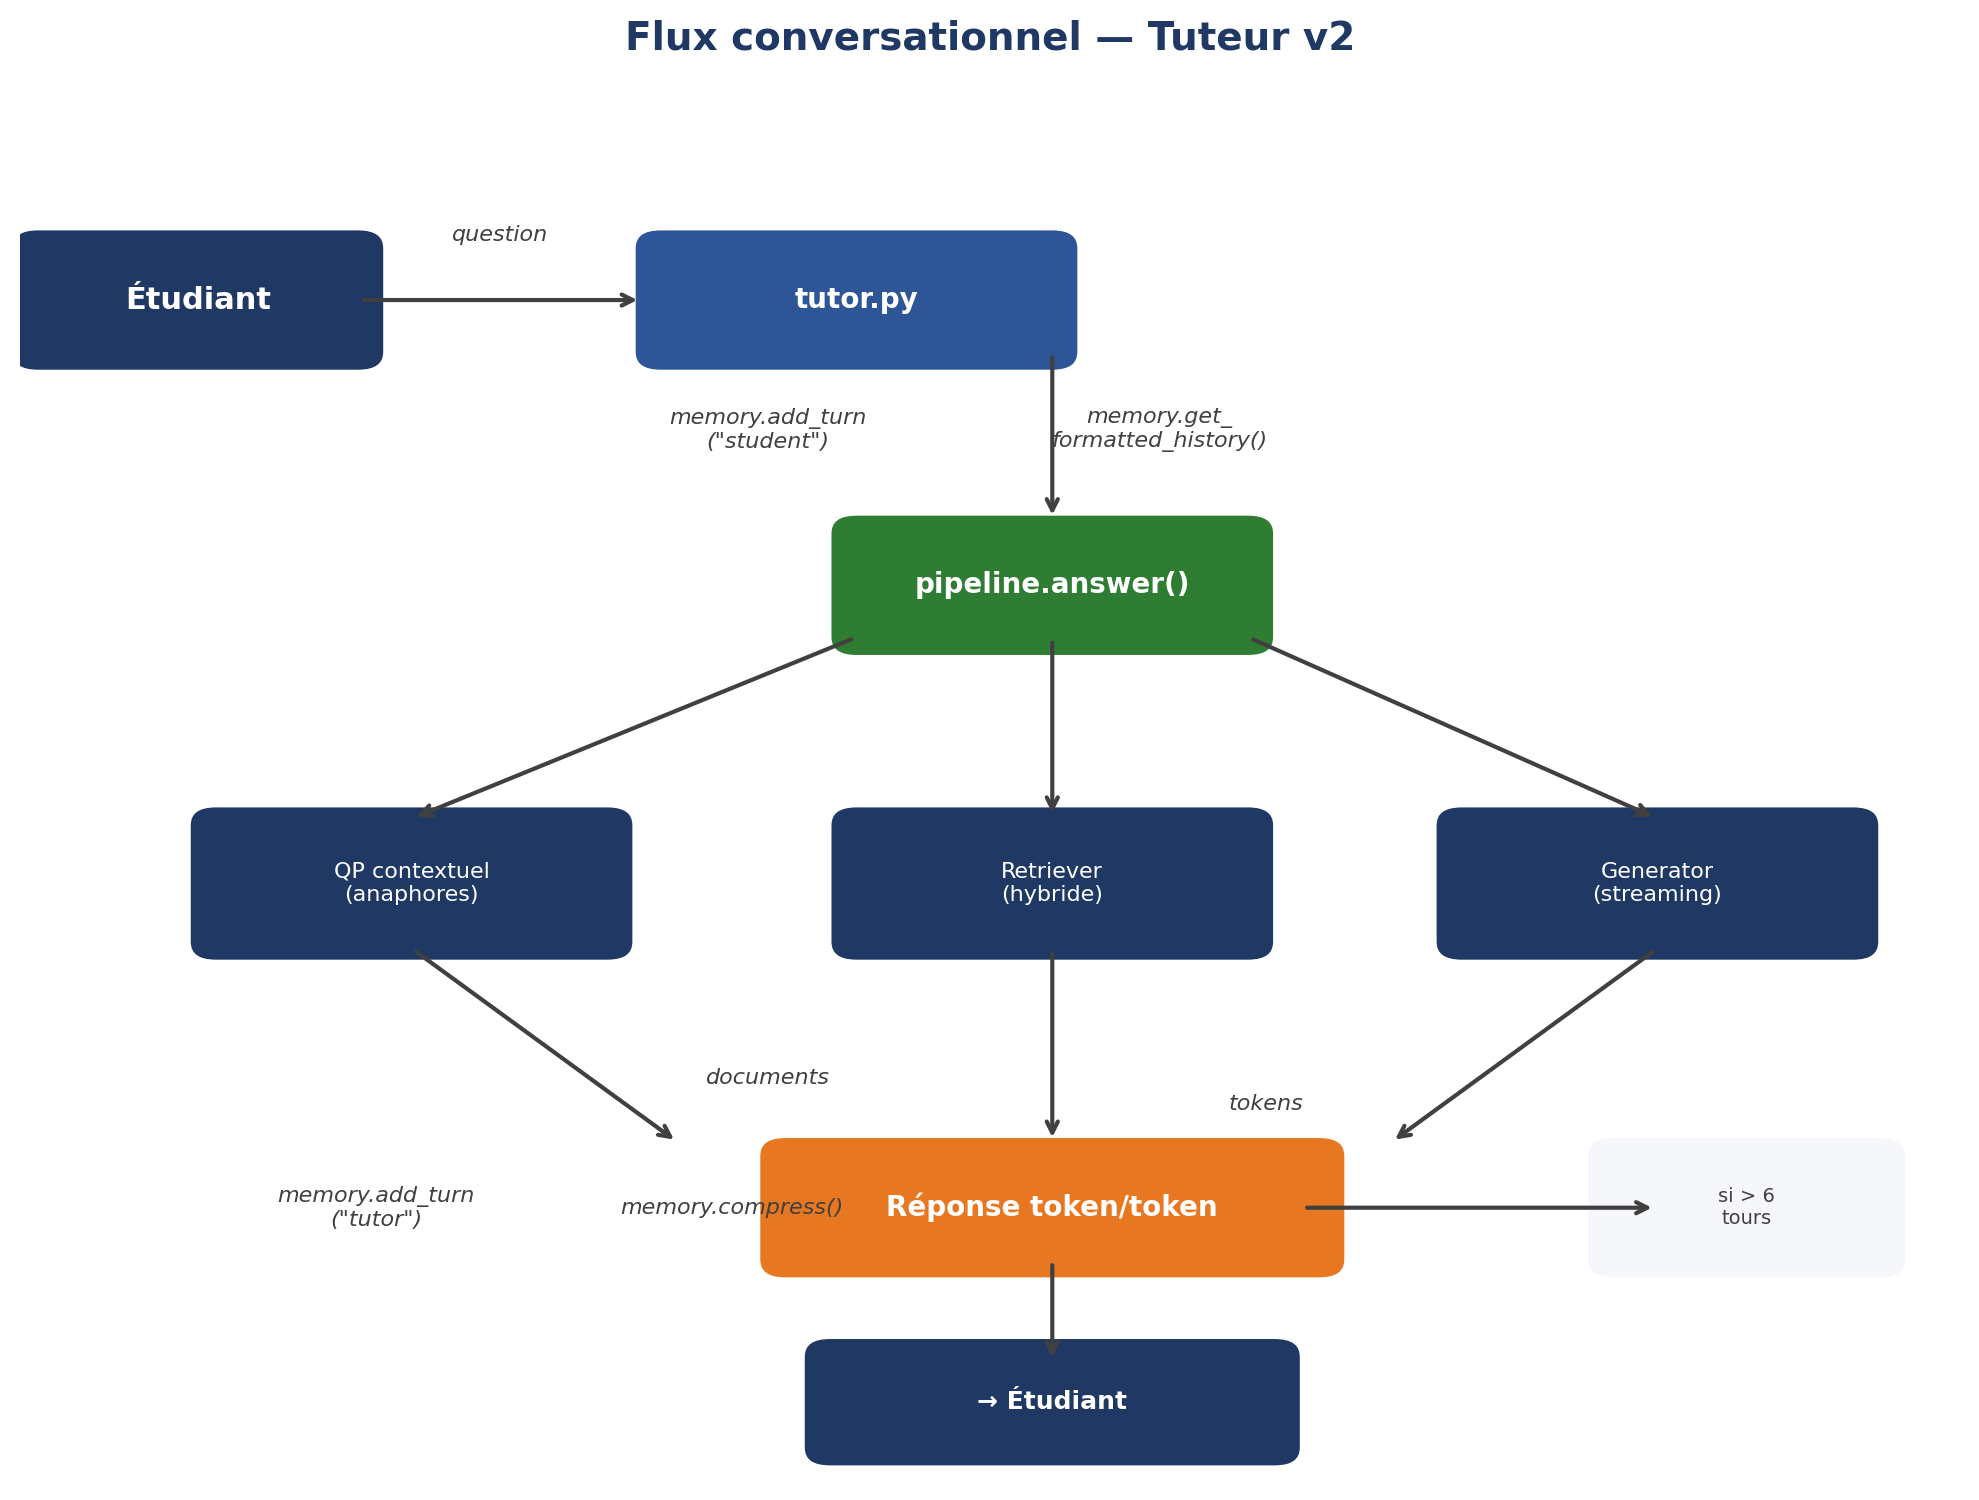
\includegraphics[width=\textwidth]{images/fig_flux_conversationnel.png}
\caption{Flux d'une requête en mode tuteur conversationnel (v2).}
\label{fig:flux-conversationnel}
\end{figure}

La mémoire conversationnelle est implémentée dans le module \texttt{conversation/memory.py} via la classe \texttt{ConversationMemory}. Le pipeline sous-jacent reste strictement \textit{stateless} : il reçoit l'historique sous forme de chaîne formatée, sans avoir connaissance de la gestion de la mémoire.

\subsubsection{Stockage et compression}

La mémoire utilise une stratégie de \textbf{fenêtre glissante avec résumé}, inspirée des architectures de mémoire longue dans les systèmes conversationnels modernes :

\begin{table}[H]
\centering
\begin{tabularx}{\linewidth}{L{4cm} L{8cm}}
\toprule
\rowcolor{bleuPrincipal}
\textcolor{white}{\textbf{État}} & \textcolor{white}{\textbf{Comportement}} \\
\midrule
$\leq$ \texttt{recent\_window} (défaut : 6) & Aucune compression --- tous les tours sont gardés intacts \\
$>$ \texttt{recent\_window} & Les tours anciens sont résumés par \texttt{qwen2.5:14b} (temperature=0) en 2--3 phrases. Les \texttt{recent\_window} derniers restent intacts \\
Échec du summarizer LLM & Fallback : troncature simple à \texttt{max\_summary\_tokens} mots (défaut : 500) \\
Historique $>$ 4000 tokens & Les tours les plus anciens sont supprimés (minimum 2 préservés) \\
\bottomrule
\end{tabularx}
\caption{Stratégie de compression de la mémoire conversationnelle.}
\label{tab:memoire-compression}
\end{table}

\begin{figure}[H]
\centering
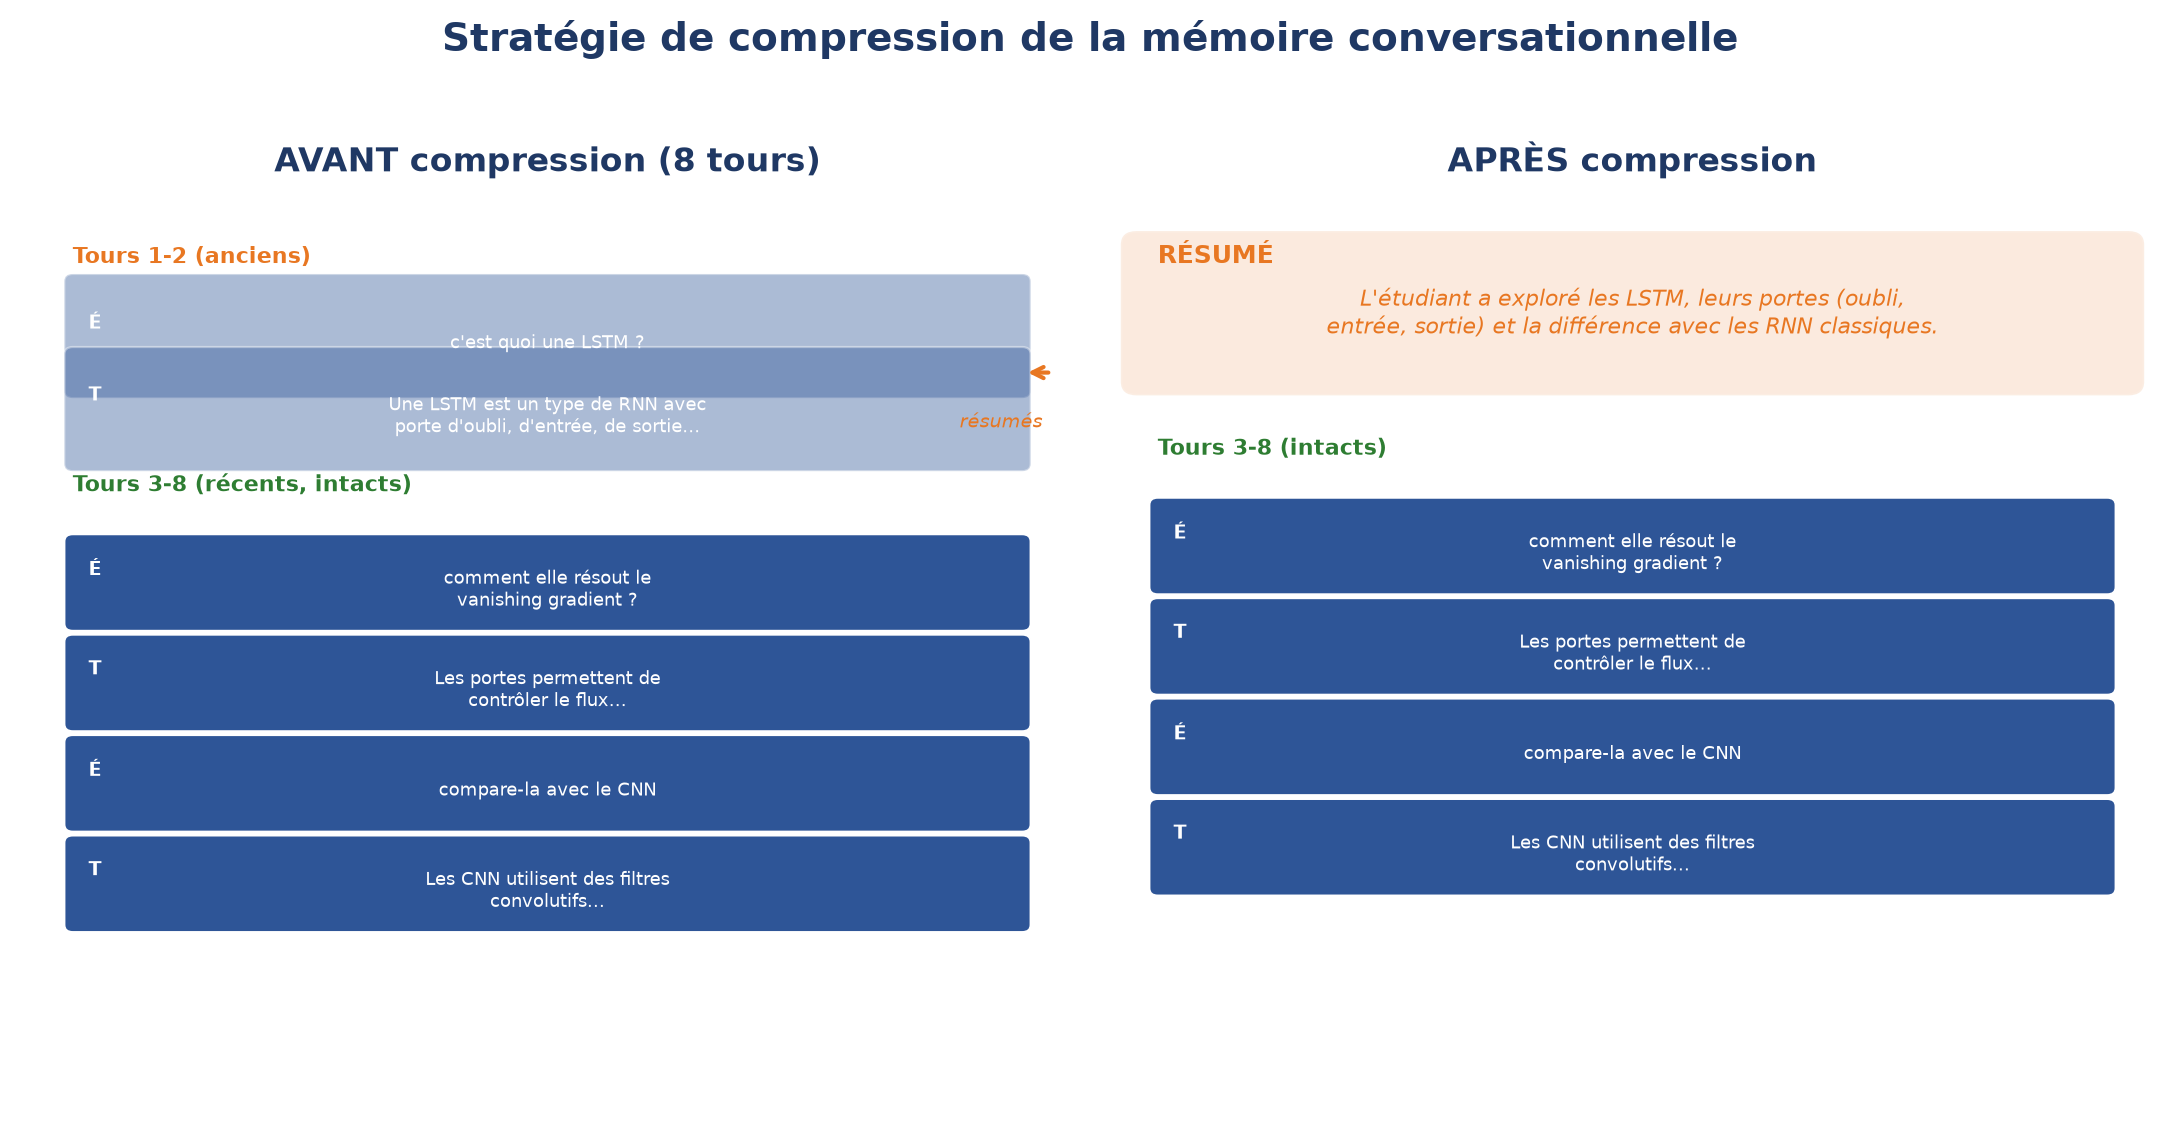
\includegraphics[width=\textwidth]{images/fig_compression_memoire.png}
\caption{Illustration de la stratégie de compression : avant (8 tours) et après résumé LLM.}
\label{fig:compression-memoire}
\end{figure}

Le résumé par LLM produit des synthèses denses et pertinentes. Par exemple, après plusieurs tours d'échange sur les LSTM, le résumé capture l'essentiel : \textit{<< L'étudiant a exploré les LSTM, leurs portes (oubli, entrée, sortie) et la différence avec les RNN classiques. >>}

\subsubsection{Formatage et injection dans le prompt}

L'historique formaté est injecté dans le prompt de génération \textbf{avant} les documents de cours. Cette structure permet au LLM de comprendre le contexte conversationnel avant de consulter les documents, ce qui est essentiel pour résoudre les références implicites (anaphores, ellipses).

\begin{lstlisting}[caption={Structure du prompt en mode conversationnel}, label={lst:prompt-conversation}]
HISTORIQUE DE LA CONVERSATION :
[RÉSUMÉ] résumé des tours anciens (si disponibles)
[DERNIERS ÉCHANGES] 6 derniers tours intacts

DOCUMENTS DE COURS DISPONIBLES :
[\S{}10.1 -- LSTM] ...  [\S{}7.1 -- CNN] ...

QUESTION DE L'ÉTUDIANT :
<question originale>
\end{lstlisting}

\subsection{Prompt socratique}

Le prompt du tuteur (\texttt{TUTOR\_SYSTEM\_PROMPT}, dans \texttt{conversation/prompts.py}) diffère fondamentalement du prompt professeur utilisé pour l'évaluation (\texttt{DEFAULT\_SYSTEM\_PROMPT}) :

\begin{table}[H]
\centering
\begin{tabularx}{\linewidth}{L{4.5cm} L{4cm} L{4cm}}
\toprule
\rowcolor{bleuPrincipal}
\textcolor{white}{\textbf{Aspect}} &
\textcolor{white}{\textbf{Professeur (v1)}} &
\textcolor{white}{\textbf{Tuteur (v2)}} \\
\midrule
\textbf{Posture}    & Réponse directe et factuelle & Expliquer, puis relancer \\
\textbf{Structure}  & Une réponse, pas de dialogue & Deux temps : explication + question \\
\textbf{Adaptation} & Aucune                      & Détection du niveau (débutant/intermédiaire/avancé) \\
\textbf{Erreur}     & Non gérée                   & \textit{<< Presque ! Il y a une nuance... >>} \\
\textbf{Blocage}    & Non géré                    & Simplification avec analogie \\
\textbf{Ancrage}    & Citations [\S{}X.Y]            & Citations [\S{}X.Y] (identique) \\
\textbf{Refus}      & Phrase de refus stricte     & Phrase de refus stricte (identique) \\
\bottomrule
\end{tabularx}
\caption{Comparaison des deux prompts du système.}
\label{tab:prompts}
\end{table}

Les règles d'ancrage documentaire et de refus sont \textbf{identiques} entre les deux prompts --- seule la posture pédagogique change. Cette séparation garantit que l'évaluation quantitative (réalisée avec le prompt professeur) reste valide et comparable, indépendamment du comportement interactif du tuteur.

\subsection{Streaming token par token}

Le mode conversationnel introduit le streaming des réponses : les tokens sont affichés au fur et à mesure de leur génération, plutôt que d'attendre la réponse complète. Cette fonctionnalité, absente de la v1 (qui utilisait un appel bloquant), améliore significativement l'expérience utilisateur en réduisant la latence perçue.

Le streaming est implémenté via \texttt{chat\_stream()} dans \texttt{llm\_client.py} et exposé via le paramètre \texttt{stream=True} de \texttt{pipeline.answer()}. Le pipeline gère automatiquement la consommation du générateur de tokens et la reconstitution de la réponse complète.

\textbf{Limitation} : en mode streaming, le mécanisme de refus post-génération (M2, \texttt{verify\_answer}) est désactivé car il nécessite la réponse complète. Seul le M1 (score du reranker) protège contre les réponses hors-contexte en mode conversationnel.

\subsection{Query processing contextuel}
\label{sec:qp-contextuel}

Dans la version 2 initiale, le \textit{query processing} (reformulation et décomposition de la question) opérait sans connaissance de l'historique de conversation. Une question comme \textit{<< compare-la avec le CNN >>} était reformulée sans savoir que le pronom \textit{<< la >>} désignait une LSTM. Le LLM comprenait la référence uniquement via l'historique injecté dans le prompt de génération --- mais le \textit{retrieval}, qui intervient avant la génération, utilisait une requête ambiguë.

La version 2 finale introduit le \textbf{\textit{query processing} contextuel} : l'historique de conversation est désormais transmis au module \texttt{process\_query()} en plus du \texttt{generator}. Le system prompt du QP a été enrichi pour instruire le LLM de résoudre les anaphores et références implicites avant la reformulation.

\begin{lstlisting}[caption={Transmission de l'historique au QP (pipeline.py)}, label={lst:qp-contextuel}]
# Avant (v2 initiale)
proc = process_query(query)

# Après (v2 finale)
proc = process_query(query, history=history)
\end{lstlisting}

Le module \texttt{query\_processing.py} injecte l'historique dans le prompt utilisateur lorsque celui-ci est fourni :

\begin{lstlisting}[caption={Injection de l'historique dans le QP (query\_processing.py)}, label={lst:qp-history-inject}]
def process_query(query, history=None, model=None):
    if history:
        user_message = (
            f"HISTORIQUE DE CONVERSATION :\n{history}\n\n"
            f"QUESTION A REFORMULER :\n{query}"
        )
    else:
        user_message = query
    raw = chat(_SYSTEM_PROMPT, user_message)
\end{lstlisting}

Le system prompt du QP inclut désormais une instruction explicite de résolution d'anaphores : \textit{<< Si un HISTORIQUE DE CONVERSATION est fourni, utilise-le pour résoudre les références implicites (pronoms, anaphores, ellipses) AVANT de reformuler. >>}

L'impact de cette amélioration est analysé dans la section validation (\ref{sec:validation-qp}).

\subsection{Limites actuelles de la v2}

\begin{itemize}
  \item \textbf{M2 désactivé en streaming} : la vérification post-génération nécessite la réponse complète et n'est pas exécutée en mode streaming. Seul le M1 protège activement contre les réponses hors-contexte en mode conversationnel.

  \item \textbf{Score reranker limité par le contenu du corpus} : le QP contextuel résout correctement les anaphores (cf. section~\ref{sec:validation-qp}), mais le score du cross-encoder reste limité par l'absence de contenu explicitement comparatif dans le corpus. L'enrichissement du corpus avec des sections dédiées aux comparaisons d'architectures améliorerait les scores sur les questions de type follow-up comparatif.

  \item \textbf{Évaluation multi-tour absente} : les métriques actuelles (Hit@k, MRR, refus) sont conçues pour un dataset de questions isolées. Une évaluation spécifique au multi-tour (métriques de rétention de contexte, de cohérence inter-tours) reste à développer.
\end{itemize}

\subsection{Bilan de l'évolution v1 $\rightarrow$ v2}

Le Tableau~\ref{tab:bilan-v2} synthétise les ajouts de la version 2.

\begin{table}[H]
\centering
\begin{tabularx}{\linewidth}{L{4.8cm} C{2.5cm} C{2.5cm} L{3cm}}
\toprule
\rowcolor{bleuPrincipal}
\textcolor{white}{\textbf{Capacité}} &
\textcolor{white}{\textbf{v1}} &
\textcolor{white}{\textbf{v2}} &
\textcolor{white}{\textbf{Module}} \\
\midrule
Mémoire conversationnelle      & Non           & Oui (fenêtre + résumé LLM) & \texttt{conversation/memory.py} \\
Posture pédagogique            & Professeur    & Tuteur socratique          & \texttt{conversation/prompts.py} \\
Streaming                      & Non (bloc)    & Oui (token/token)          & \texttt{llm\_client.py} \\
QP contextuel                  & Non           & Oui (résolution anaphores) & \texttt{query\_processing.py} \\
Citations lisibles             & [DOC X] (opaque) & [\S{}X.Y] (section du cours) & \texttt{generator.py}, prompts \\
Évaluation par question        & Non           & Oui (3 niveaux)            & \texttt{evaluation/per\_question.py} \\
Compression automatique        & ---           & Oui (LLM summarizer)       & \texttt{conversation/memory.py} \\
Interface                      & \texttt{chat.py} & \texttt{chat.py} + \texttt{tutor.py} & \texttt{cli/} \\
\bottomrule
\end{tabularx}
\caption{Bilan de l'évolution v1 $\rightarrow$ v2.}
\label{tab:bilan-v2}
\end{table}

\subsection{Validation expérimentale}
\label{sec:validation-v2}

Pour valider le fonctionnement du tuteur conversationnel, une session de test a été conduite sur deux questions consécutives illustrant un scénario typique d'interaction étudiant-tuteur : une question initiale ouverte, suivie d'une question de suivi avec référence implicite. Les métriques présentées ci-dessous sont calculées en temps réel par le module \texttt{--show-eval}, sans référence annotée : score du reranker (qualité du retrieval), nombre de contextes et parents uniques (diversité), overlap lexical (recouvrement question$\leftrightarrow$contextes), volume des contextes et temps de génération.

\subsubsection{Question 1 : question initiale}

La première question est une demande d'explication ouverte : \textit{<< c'est quoi une LSTM ? >>}. Le système doit retrouver les passages pertinents, générer une explication structurée avec citations, et terminer par une relance socratique.

\begin{table}[H]
\centering
\begin{tabularx}{\linewidth}{L{3.5cm} L{2.5cm} L{6cm}}
\toprule
\rowcolor{bleuPrincipal}
\textcolor{white}{\textbf{Métrique}} & \textcolor{white}{\textbf{Valeur}} & \textcolor{white}{\textbf{Commentaire}} \\
\midrule
Score reranker (top)     & 0,986  & Excellent : le meilleur contexte est très pertinent \\
Score reranker (moy, étendue) & 0,855 [0,798--0,986] & Les 4 contextes sont de bonne qualité, distribution serrée \\
Contextes               & 4 (4 parents uniques) & Aucun doublon, bonne diversité \\
Refus                   & Non    & Décision correcte \\
Longueur réponse        & 1 280 car. & Réponse complète et structurée \\
Temps de génération     & 4,0 s  & Confortable pour l'interactif \\
\bottomrule
\end{tabularx}
\caption{Métriques d'évaluation --- Question 1 (question initiale).}
\label{tab:session-q1}
\end{table}

\subsubsection{Question 2 : suivi avec référence implicite}

La seconde question est un follow-up : \textit{<< compare-la avec le CNN >>}. Sans mémoire conversationnelle, le pronom \textit{<< la >>} serait inintelligible pour le système. Avec la mémoire active, le tuteur comprend que la référence désigne la LSTM du tour précédent.

\begin{table}[H]
\centering
\begin{tabularx}{\linewidth}{L{3.5cm} L{2.5cm} L{6cm}}
\toprule
\rowcolor{bleuPrincipal}
\textcolor{white}{\textbf{Métrique}} & \textcolor{white}{\textbf{Valeur}} & \textcolor{white}{\textbf{Commentaire}} \\
\midrule
Query processing         & 1 reformulée + 2 sous-questions & La décomposition fonctionne malgré une question courte \\
Score reranker (top)     & 0,488  & Correct mais 2$\times$ plus faible que Q1 --- attendu pour une question comparative \\
Score reranker (moy, étendue) & 0,336 [0,145--0,494] & Le sujet << CNN vs LSTM >> est plus dispersé dans le corpus \\
Contextes               & 4 (4 parents uniques) & Bonne diversité malgré des scores plus bas \\
Volume contextes        & 13 513 car. & Contexte abondant, compense les scores moyens \\
Longueur réponse        & 2 987 car. & Réponse très complète (comparaison structurée) \\
Temps de génération     & 8,6 s  & Acceptable pour une réponse longue \\
\bottomrule
\end{tabularx}
\caption{Métriques d'évaluation --- Question 2 (suivi avec référence implicite).}
\label{tab:session-q2}
\end{table}

\subsubsection{Analyse des résultats}

Cette session de validation met en évidence trois points :

\begin{enumerate}
  \item \textbf{La mémoire conversationnelle fonctionne} : le tuteur a correctement interprété la question de suivi en résolvant la référence implicite grâce à l'historique.

  \item \textbf{Le score reranker baisse sur les follow-ups} : 0,986 $\rightarrow$ 0,488. Cette dégradation est attendue pour les questions comparatives, qui mobilisent des passages plus dispersés dans le corpus. Le \textit{query processing} compense partiellement en générant des sous-questions plus ciblées.

  \item \textbf{L'évaluation en temps réel est un outil de diagnostic} : sans \texttt{--show-eval}, la baisse de qualité du retrieval entre Q1 et Q2 serait invisible. Le rapport par question rend cette information accessible et actionnable pour l'amélioration du retriever.
\end{enumerate}

\subsubsection{Impact du QP contextuel}
\label{sec:validation-qp}

Pour mesurer l'effet du \textit{query processing} contextuel (section~\ref{sec:qp-contextuel}), la même session de test a été exécutée avant et après l'activation de cette fonctionnalité. Le Tableau~\ref{tab:qp-comparaison} présente les résultats comparés pour la question de suivi (Q2).

\begin{table}[H]
\centering
\begin{tabularx}{\linewidth}{L{3.5cm} L{3cm} L{3cm} L{3cm}}
\toprule
\rowcolor{bleuPrincipal}
\textcolor{white}{\textbf{Métrique}} &
\textcolor{white}{\textbf{Sans QP contextuel}} &
\textcolor{white}{\textbf{Avec QP contextuel}} &
\textcolor{white}{\textbf{Delta}} \\
\midrule
Score reranker (top)     & 0,488 & 0,491 & +0,003 (quasi identique) \\
Score reranker (moy)     & 0,336 & 0,294 & $-$0,042 \\
Overlap lexical          & 0\,\% (0/1) & \textbf{100\,\% (2/2)} & \textbf{+100 pts} \\
Requête reformulée       & <<~Comparez les réseaux...~>> (vague) & <<~Comparer les performances LSTM vs CNN~>> (désambiguïsée) & Anaphore résolue \\
Temps de génération      & 8,6 s & 12,8 s & +4,2 s \\
\bottomrule
\end{tabularx}
\caption{Comparaison avant/après activation du QP contextuel sur la question de suivi Q2.}
\label{tab:qp-comparaison}
\end{table}

Deux enseignements se dégagent de cette comparaison :

\begin{enumerate}
  \item \textbf{L'anaphore est résolue} : l'overlap lexical passe de 0\,\% à 100\,\%, confirmant que la requête reformulée contient désormais les termes explicites (LSTM, CNN) présents dans les contextes. La requête reformulée mentionne explicitement <<~LSTM~>> et <<~CNN~>> là où la version sans QP contextuel produisait une formulation vague.

  \item \textbf{Le score reranker n'augmente pas} : malgré une requête parfaitement désambiguïsée, le score du cross-encoder reste stable (0,488 $\rightarrow$ 0,491). Ce résultat indique que le facteur limitant n'est pas la qualité de la requête, mais le \textbf{contenu du corpus lui-même} : le cours ne contient pas de section dédiée à la comparaison directe des architectures LSTM et CNN. Les passages récupérés décrivent chaque architecture séparément, et le cross-encoder leur attribue des scores moyens car ils ne répondent que partiellement à la question comparative. L'amélioration du retrieval sur les follow-ups comparatifs nécessiterait donc un enrichissement du corpus plutôt qu'une amélioration du QP.
\end{enumerate}
